% https://da.overleaf.com/latex/templates/cs310-assignment-template/qrqpndrxpcht
%%%%%%%%%%%%%%%%% DO NOT CHANGE HERE %%%%%%%%%%%%%%%%%%%% {
\documentclass[12pt,letterpaper]{article}
\usepackage{fullpage}
\usepackage[top=2cm, bottom=4.5cm, left=2.5cm, right=2.5cm]{geometry}
\usepackage{amsmath,amsthm,amsfonts,amssymb,amscd}
\usepackage{lastpage}
\usepackage{enumerate}
\usepackage{fancyhdr}
\usepackage{mathrsfs}
\usepackage{xcolor}
\usepackage{graphicx}
\usepackage{listings}
\usepackage{hyperref}
\usepackage{listings}
\usepackage{float}
\usepackage{wrapfig}

\hypersetup{%
  colorlinks=true,
  linkcolor=blue,
  linkbordercolor={0 0 1}
}

\renewcommand{\labelenumii}{\theenumii}
\renewcommand{\theenumii}{\theenumi.\arabic{enumii}.}

\setlength{\parindent}{0.0in}
\setlength{\parskip}{0.05in}
%%%%%%%%%%%%%%%%%%%%%%%%%%%%%%%%%%%%%%%%%%%%%%%%%%%%%%%%%% }

%%%%%%%%%%%%%%%%%%%%%%%% CHANGE HERE %%%%%%%%%%%%%%%%%%%% {
\newcommand\course{BDSA2021}
\newcommand\semester{\today}
\newcommand\hwnumber{01}         % <-- ASSIGNMENT #
\newcommand\NetIDa{Andreas Wachs Hjalager}      % <-- YOUR NAME
\newcommand\NetIDb{19167}      % <-- STUDENT ID #
%%%%%%%%%%%%%%%%%%%%%%%%%%%%%%%%%%%%%%%%%%%%%%%%%%%%%%%%%% }

%%%%%%%%%%%%%%%%% DO NOT CHANGE HERE %%%%%%%%%%%%%%%%%%%% {
\pagestyle{fancyplain}
\headheight 35pt
\lhead{\NetIDa}
\lhead{\NetIDa\\Student ID: \NetIDb}
\chead{\textbf{\Large Assignment \hwnumber}}
\rhead{\course \\ \semester}
\lfoot{}
\cfoot{}
\rfoot{\small\thepage}
\headsep 1.5em
%%%%%%%%%%%%%%%%%%%%%%%%%%%%%%%%%%%%%%%%%%%%%%%%%%%%%%%%%% }

\lstdefinestyle{sharpc}{language=[Sharp]C}
\lstset{style=sharpc}

\begin{document}
\section{The leap year algorithm}
The \textit{leap year algorithm} calculates whether or not a given year is a leap year or not.

\begin{wrapfigure}[37]{r}{0.35\textwidth}
  \begin{center}
   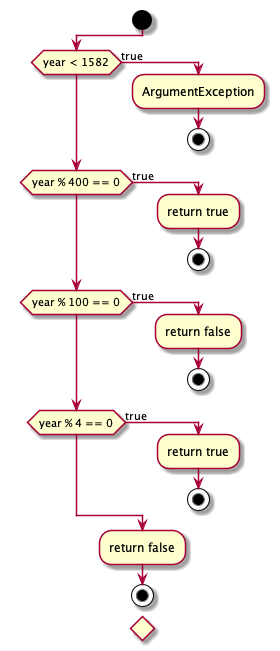
\includegraphics[scale=0.6]{./images/isleapyear_algorithm.png}
  \end{center}
  \caption{\textit{The leap year algorithm}}
\end{wrapfigure}

The algorithm is contained within a single function, that takes an integer as a parameter.

The input goes through a series of judgements and immediately returns when the first check is deemed to be \lstinline{true}
\begin{enumerate}
    \item The first judgement is the check to see if the number is greater than $1582$.
          \begin{enumerate}
              \item If true, the algorithm returns an ArgumentException, as it is not a valid input.
              \item Otherwise the judging moves along
          \end{enumerate}
    \item The year input is divisible by 400
          \begin{enumerate}
              \item If true, the algorithm deems the year to be a leap year (returns true)
              \item Otherwise the judging moves along
          \end{enumerate}
    \item The year input is divisible by 100
          \begin{enumerate}
              \item If true, the algorithm deems the year to \textbf{not} be a leap year (returns false)
              \item Otherwise the judging moves along
          \end{enumerate}
    \item The year input is divisible by 4
          \begin{enumerate}
              \item If true, the algorithm deems the year to be a leap year (returns true)
              \item Otherwise the judging moves along
          \end{enumerate}
    \item If true, the algorithm deems the year to \textbf{not} be a leap year (returns false)
\end{enumerate}





\pagebreak
\section{Source code}
\begin{lstlisting}[breaklines=true] 
  public static bool IsLeapYear(int year)
    {
      if (year < 1582)
      {
        throw new ArgumentException($"the input year \"#{year}\" should be greater or equal to 1582");
      }
      else if (year % 400 == 0)
      {
        return true;
      } 
      else if (year % 100 == 0)
      {
        return false;
      } 
      else if (year % 4 == 0)
      {
        return true;
      } 
      else
      {
        return false;
      }
    }
\end{lstlisting}

\end{document}

  